\documentclass{beamer}
\usepackage[utf8]{inputenc}
\usepackage[T1]{fontenc}
\usepackage{lmodern}
\usepackage{listings}
\usepackage{xcolor}
\usepackage{tikz}
\usetikzlibrary{positioning, arrows.meta}

\usetheme{Madrid}
\setbeamertemplate{navigation symbols}{}
\setbeamertemplate{footline}{}

\title[Git Basics]{Git: Version Control System}
\author[Alessio]{Alessio}
\date{\today}

\begin{document}

\begin{frame}
  \titlepage
\end{frame}

\begin{frame}{What is Git?}
  \begin{itemize}
    \item Git is a distributed version control system.
    \item It tracks changes in the project over time.
    \item It helps teamwork without losing updates.
    \item Each saved change is a \textbf{commit}.
  \end{itemize}

  \vspace{0.2cm}
  \begin{center}
    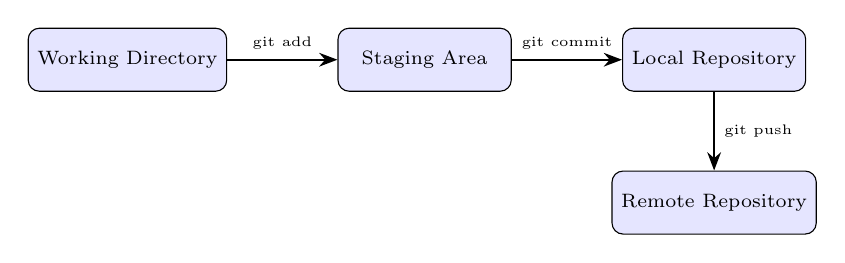
\begin{tikzpicture}[
      box/.style={draw, rounded corners, fill=blue!10, minimum width=2.2cm, minimum height=0.8cm, align=center, font=\scriptsize},
      arrow/.style={->, thick, >=Stealth}
    ]
      \node[box] (wd) {Working Directory};
      \node[box, right=1.4cm of wd] (stage) {Staging Area};
      \node[box, right=1.4cm of stage] (repo) {Local Repository};
      \node[box, below=1.0cm of repo] (remote) {Remote Repository};

      \draw[arrow] (wd) -- node[above, font=\tiny]{git add} (stage);
      \draw[arrow] (stage) -- node[above, font=\tiny]{git commit} (repo);
      \draw[arrow] (repo) -- node[right, font=\tiny]{git push} (remote);
    \end{tikzpicture}
  \end{center}

  \vspace{0.15cm}
  \begin{block}{Why use it?}
    \begin{itemize}
      \item Recover previous versions
      \item Work on multiple features
      \item Collaborate safely
      \item Avoid overwriting others
    \end{itemize}
  \end{block}
\end{frame}

\begin{frame}[fragile]{Main commands}
  \scriptsize
  \begin{lstlisting}[language=bash]
# initialize repo
$ git init

# status
$ git status

# add files
$ git add file_name

# commit
$ git commit -m "message"

# list branches
$ git branch

# new branch
$ git checkout -b new_feature
  \end{lstlisting}

  \vspace{0.15cm}
  \begin{alertblock}{Key idea}
    A repository keeps project history, while branches let you work independently from the main version.
  \end{alertblock}
\end{frame}

\end{document}
